% !TEX TS-program = xelatex
% !BIB program = bibtex
% !TEX encoding = UTF-8 Unicode

\documentclass[
  twoside,                          % oneside | twoside
  openright,                        % openright
  degree    = master,               % degree = master | doctor
  language  = english,              % language = chinese | english
  fontset   = default,              % fontset = default | template | system | overleaf
  watermark = true,                 % watermark = true | false
  watermarkcolor = true,            % watermarkcolor = true | false
  doi       = true,                 % doi = true | false
  colorlinks = true,                % colorlink = true | false
]{ntuthesis}

% !TeX root = ./main.tex

% --------------------------------------------------
% 資訊設定(Information Configs)
% --------------------------------------------------

\ntusetup{
  university*   = {National Taiwan University},
  university    = {國立臺灣大學},
  college       = {理學院},
  college*      = {College of Science},
  institute     = {物理學研究所},
  institute*    = {Department of Physics},
  title         = {尋找Belle II中$B$介子三體衰變至$K$介子與二體$\pi$介子},
  title*        = {Search for $B^+\to K^+\pi^+\pi^-$ decay at Belle II},
  author        = {梁祐瑄},
  author*       = {You-Hsuan Liang},
  ID            = {R07222059},
  advisor       = {張寶棣},
  advisor*      = {Paoti Chang},
  profession    = {教授},
  date          = {2021-08-30},         % 若註解掉,則預設為當天
  oral-date     = {2021-07-30},         % 若註解掉,則預設為當天
  DOI           = {10.9487/NTU202109487},
  keywords      = {Belle II實驗, $B$介子, 衰變},
  keywords*     = {Belle II, $B$ meson, $B$ decay},
}

% --------------------------------------------------
% 加載套件(Include Packages)
% --------------------------------------------------

%\usepackage[sort&compress]{natbib}      % 參考文獻
\usepackage{amsmath, amsthm, amssymb}   % 數學環境
\usepackage{ulem, CJKulem}              % 下劃線、雙下劃線與波浪紋效果
\usepackage{booktabs}                   % 改善表格設置
\usepackage{multirow}                   % 合併儲存格
\usepackage{diagbox}                    % 插入表格反斜線
\usepackage{array}                      % 調整表格高度
\usepackage{longtable}                  % 支援跨頁長表格
\usepackage{paralist}                   % 列表環境
\usepackage{makecell}                   % 製作細胞格
\usepackage{hologo}                  % 提供各種logo

\usepackage{lipsum}                     % 英文亂字
\usepackage{zhlipsum}                   % 中文亂字

% --------------------------------------------------
% 套件設定(Packages Settings)
% --------------------------------------------------

\def\arraystretch{2} % 表格使用2倍行高 
% 定義三種新的column
\renewcommand{\tabularxcolumn}[1]{>{\small}m{#1}}
\newcolumntype{L}{>{\raggedright\arraybackslash}X} % 靠左對齊 自動換行
\newcolumntype{R}{>{\raggedleft\arraybackslash}X}  % 靠左對齊 自動換行
\newcolumntype{C}{>{\centering\arraybackslash}X}   % 置中對齊 自動換行

% 不要加上header的橫線
\renewcommand{\headrulewidth}{0pt}
\renewcommand{\footrulewidth}{0pt}

\begin{document}

% 封面與口試審定
% Cover and Verification Letter
\makecover                          % 論文封面(Cover)
\makeverification{figures/verificationletter.pdf} % 口試委員審定書(Verification Letter)

% 致謝與論文摘要
% Acknowledgement and Abstract
% !TeX root = ../main.tex

% 英文誌謝
\begin{acknowledgement*}

I often eat at foreign friends' houses. When the candles are lit, the dishes are ready, and the host is in place, the host’s little boy or girl always raises his little hand, bows his head to thank God for the gift, and welcomes the guest.

When I first arrived in the United States, I was often embarrassed. Because of the habit developed in the country, I started before sitting down.

In the future, when you go to a friend's house for dinner, always ask yourself first, don't forget today, don't start too fast! In the past few years, I have become very used to it. But I always think that it is just a different kind of custom ceremony. In my opinion, forgetting or not forgetting does not matter much.

Once the year before last, I went to eat at the same house again. But this time, the host’s grandmother thanked him for the meal. Her snow-white hair, trembling voice, under the flickering candlelight, reminded me of my childhood grandmother. That night, I suddenly felt that my calm and watery emotions turned up against the huge waves.

When I was young, every winter night, our big family gathered around a big round table to eat. I always sit next to my grandmother, who always touches my head and says, "God rewards our family for a full meal. Remember, no grain of rice is allowed in the rice bowl. If the food is spoiled, God will not give us food. Up."

When I just started elementary school, my righteous thoughts brought down idols and dispelled superstitions. My school was the former Guandi Temple, and my desk was the offering table. I once drew glasses for Zhou Cang and a beard for Guan Ping. My grandmother's words, God, I think it is redundant and outdated.

However, I respect my grandparents very much, because they really earned the food, and they did set up this family.

I thank the grandparents in front of me, and I don't have to thank the vague God.

This idea has not changed with age. How many years have passed in this philosophy.

After dinner in this foreign family, because of this old foreign lady, I think of my childhood; because of my childhood, I think of a series of very strange phenomena.

Grandfather gritted his teeth in the wind and rain every year, and grandmother gritted his teeth in the tea and rice every year. They knew that they had to drip the sweat from their eyebrows to pick up the wheat ears in the field. Why did they thank God? I am obviously a kid, eating and playing, but why don't I thank God?

This strange state of mind has always been a mystery in my heart.

Until the year before last, when I was in Princeton, I browsed Einstein's "The World I Seen" and got new insights.

This is a non-scientific collection of essays, specifically containing some of Einstein's speeches at the memorial, the welcome party, and the funeral of a friend.

When I was reading this book, I suddenly discovered that Einstein wanted to give the audience an impression as much as possible: that is, his contribution was either due to A or B, and was not very relevant to Einstein himself.

Even the new and original special theory of relativity that has been created since ancient times has no reference to quote, but it flew in the last sky, "Thanks to my colleague and friend Besso for the discussion of the phase."

Other articles, such as the general theory of relativity, which has been struggling for more than ten years, are partly promoted to the cooperation of friends in the past; this kind of humility, this kind of no credit is rare in the history of science.

I just thought, I can't live so much, why? Like Einstein to the theory of relativity, like my grandmother to my family.

After several years of running around, doing some research, writing a few academic articles, and really making some small contributions, I have a new consciousness: that is, no matter what, too many people get it, and it’s out of it. There are too few people who own it.

Because there are too many people to thank, just thank God. No matter what, it doesn't need the love and inheritance of the ancestors, it needs the support and cooperation of everyone, and also wait for the opportunity to come. The more I have done something, the more I feel that my contribution is small.

As a result, entrepreneurs will naturally think of God, but the prodigal will always think of themselves.

The introduction of the introduction does not say the price, the price is also the same. This is the most perfect story composed of one of our most perfect personality in China. Why didn't Jie Zhitui say anything, because he felt that the merits of greed for the heavens were his own power, which a gentleman would disdain and should not do.

When Einstein first arrived in Princeton, the director discussed with him the issue of remuneration. He said five thousand. The director said, "I give you five thousand, how can I give a college graduate? It's still fifteen thousand yuan!" Isn't this a foreign recommendation?

Why did Jie Zhitui and Einstein specialize in such stupid things? Make great contributions, but don't take credit for it. They know that for doing things and meritorious service, there are more people who can cooperate with others, and fewer people who can do things by themselves. So it is natural to have a feeling of thanking everyone and God.

Let us look back and think about it, how much stronger China was in the past 50 or 60 years than when I was 7 or 8 years old! If historians write the history of our country in the past fifty or sixty years, they must name it the arrogant and naive, lawless and lawless era.

No matter which line or sector, most of them are boasting and deceiving themselves. The days are long, and even I believe it is true, and the catastrophe is terrible.

Because you haven't done any real things, haven't built any real gong, naturally you won't feel thankful.

Philosophers know that this symptom is the most terrifying, so they have created many characters and stories that know good and bad.

A person asked a writer, I remember it was Hugo, "If all the books in the world need to be burned and only one is allowed, what should be kept?" Hugo said without hesitation, "Just keep< "The Book of Job"." Job is the introduction in the "Bible". The rich also thank the heavens, the poor also thank the heavens, the sickness also thank the heavens, and the sufferings also thank the heavens.

Our ideological world is still in the chaotic and naive period, and needs Job's spirit and the enlightenment. This enlightenment is: one porridge, one meal, half a thread, half a thread, it is the crystallization of the blood and sweat of how many years and how many people. Thank you for being thankful.

\end{acknowledgement*}

% 中文誌謝
\begin{acknowledgement}

常到外國朋友家吃飯。當蠟燭燃起,菜餚布好,客主就位,總是主人家的小男孩或小女孩舉起小手,低頭感謝上天的賜予,並歡迎客人的到來。

我剛一到美時,常鬧得尷尬。因為在國內養成的習慣,還沒有坐好,就開動了。

以後凡到朋友家吃飯時,總是先囑咐自己,今天不要忘了,可別太快開動啊!幾年來,我已變得很習慣了。但我一直認為只是一種不同的風俗儀式,在我這方面看來,忘或不忘,也沒有太大的關係。

前年有一次,我又是到一家去吃飯。而這次卻是由主人家的祖母謝飯。她雪白的頭髮,顫抖的聲音,在搖曳的燭光下,使我想起兒時的祖母。那天晚上,我忽然覺得我平靜如水的情感翻起滔天巨浪來。

在小時候,每當冬夜,我們一大家人圍域個大圓桌吃飯。我總是坐在祖母身旁,祖母總是摸著我的頭說;「老天爺賞我們家飽飯吃,記住,飯碗裏一粒米都不許剩,要是糟蹋糧食,老天爺就不給咱們飯了。」

剛上小學的我,正念打倒偶像,破除迷信,我的學校就是從前的關帝廟,我的書桌就是供桌。我曾給周倉畫上眼鏡,給關平戴上鬍子,祖母的話,老天爺也者,我覺得是既多餘,又落伍的。

不過,我卻很尊敬我的祖父母,因為這飯確實是他們掙的,這家確實是他們立的。

我感謝面前的祖父母,不必感謝渺茫的老天爺。

這種想法並未因年紀長大而有任何改變。多少年,就在這種哲學中過去了。

我在這個外國家庭晚飯後,由於這位外國老太太,我想起我的兒時;由於我的兒時,我想起一串很奇怪的現象。

祖父每年在「風裏雨裏的咬牙」,祖母每年在「茶裏飯裏的自苦」,他們明明知道要滴下眉毛上的汗珠,才能撿起田中的麥穗,而為什麼要謝天?我明明是個小孩子,混吃混玩,而我為什麼卻不感謝老天爺?

這種奇怪的心理狀態,一直是我心中的一個謎。

一直到前年,我在普林斯頓,瀏覽愛因斯坦的《我所看見的世界》,得到了新的領悟。

這是一本非科學性的文集,專載些愛因斯坦在紀念會上啦、在歡迎會上啦、在朋友的葬禮中,他所發表的談話。

我在讀這本書時忽然發現愛因斯坦想盡量給聽眾一個印象:即他的貢獻不是源於甲,就是由於乙,而與愛因斯坦本人不太相干似的。

就連那篇亙古以來嶄新獨創的狹義相對論,並無參考可引,卻在最後天外飛來一筆,「感謝同事朋友貝索的時相討論。」

其他的文章,比如奮鬥苦思了十幾年的廣義相對論,數學部分推給了昔年好友的合作;這種謙抑,這種不居功,科學史中是少見的。

我就想,如此大功而竟不居,為什麼?像愛因斯坦之於相對論,像我祖母之於我家。

幾年來自己的奔波,作了一些研究,寫了幾篇學術文章,真正做了一些小貢獻以後,才有了一種新的覺悟:即是無論什麼事,得之於人者太多,出之於己者太少。

因為需要感謝的人太多了,就感謝天罷。無論什麼事,不是需要先人的遺愛與遺產,即是需要眾人的支持與合作,還要等候機會的到來。越是真正做過一點事,越是感覺自己的貢獻之渺小。

於是,創業的人,都會自然而然的想到上天,而敗家的人卻無時不想到自己。

介之推不言祿,祿亦弗及。這是我們中國的一個最完美的人格所構成的一個最完美的故事。介之推為什麼不言祿,因為他覺得貪天之功以為己力,是君子所不屑為,也是君子所不應為的。

愛因斯坦剛到普林斯頓時,主任與他商量報酬問題,他說五千。主任說:「給你五千,如何給一個大學畢業生呢?還是算一萬五千元罷!」這不是外國的介之推嗎?

為什麼介之推與愛因斯坦專幹這類傻事?立過大功,而不居功若此。他們知道作事與立功,得之於眾人合作者多,得之於自己逞能者少。於是很自然的產生一種感謝眾人、感謝上天的感覺。

我們回頭想一想,五六十年來的中國比我七八歲時的思想能強幾何!史家如果寫這五六十年來的我國歷史時,一定命名為狂妄而幼稚,無法與無天的時代。

無論哪一行、哪一界,多是自吹自擂,自欺自騙。日子長了,連自己也信以為真了,而大禍至矣。

因為沒有做任何真正的事,沒有建任何真正的功,自然而然不會有謝天的感覺。

哲學家們知道這個症候最為可怕,所以造出許多知好知歹的人物與故事來。

有一個人問一位文學家,我記得是雨果罷,「如果世界上的書全需要燒掉,而只許留一本,應留什麼?」雨果毫不猶豫的說:「只留〈約伯記〉。」約伯是《聖經》裏面的介之推,富亦謝天,貧亦謝天,病亦謝天,苦亦謝天。

我們的思想界尚在混沌幼稚時期,需要約伯的精神,需要介之推的覺悟。這個覺悟即是:一粥一飯,半絲半縷,都是多少年、多少人的血汗結晶。感謝之情,無由表達,還是謝天罷。

\end{acknowledgement}       % 致謝(Acknowledgement)
% !TeX root = ../main.tex

\begin{abstract*}

The abstract is an important component of your thesis. Presented at the beginning of the thesis, it is likely the first substantive description of your work read by an external examiner. You should view it as an opportunity to set accurate expectations.
The abstract is a summary of the whole thesis. It presents all the major elements of your work in a highly condensed form.
An abstract often functions, together with the thesis title, as a stand-alone text. Abstracts appear, absent the full text of the thesis, in bibliographic indexes such as PsycInfo. They may also be presented in announcements of the thesis examination. Most readers who encounter your abstract in a bibliographic database or receive an email announcing your research presentation will never retrieve the full text or attend the presentation.
An abstract is not merely an introduction in the sense of a preface, preamble, or advance organizer that prepares the reader for the thesis. In addition to that function, it must be capable of substituting for the whole thesis when there is insufficient time and space for the full text.

Currently, the maximum sizes for abstracts submitted to Canada's National Archive are 150 words (Masters thesis) and 350 words (Doctoral dissertation).
To preserve visual coherence, you may wish to limit the abstract for your doctoral dissertation to one double-spaced page, about 280 words.
The structure of the abstract should mirror the structure of the whole thesis, and should represent all its major elements.
For example, if your thesis has five chapters (introduction, literature review, methodology, results, conclusion), there should be one or more sentences assigned to summarize each chapter.

As in the thesis itself, your research questions are critical in ensuring that the abstract is coherent and logically structured. They form the skeleton to which other elements adhere.
They should be presented near the beginning of the abstract.
There is only room for one to three questions. If there are more than three major research questions in your thesis, you should consider restructuring them by reducing some to subsidiary status.

The most common error in abstracts is failure to present results.
The primary function of your thesis (and by extension your abstract) is not to tell readers what you did, it is to tell them what you discovered. Other information, such as the account of your research methods, is needed mainly to back the claims you make about your results.
Approximately the last half of the abstract should be dedicated to summarizing and interpreting your results.

\end{abstract*}


\begin{abstract}

一個好的摘要應該具有以下五個特點。
APA提到一篇好的摘要需有:
「精確」(accurate) :摘要應該是文章的精簡版,所以它的內容不應該超過文章內容的範圍。
「完備」(self-contained) :摘要是一篇獨立的文章,所以一些可能讓讀者讀不懂的東西不要放在摘要中;如果一定要放一些讀者讀完摘要還可能不懂的東西時,作者應該在摘要中加以解釋。例如,如果摘要中含有一些冷僻、不常見的專有名詞,則作者應該在摘要中說明名詞的定義,這樣才不會讓讀者感到生澀難懂。
「簡潔明確」(concise and specific) :字數用詞切中重點。
「非評論性」(non-evaluative) :不要在摘要中評價研究的發現。
「連貫性」及「易讀性」(coherent and readable):文章寫得很淺顯、流暢、易懂,科學報導最重要的目的是傳達信息,作者應該盡量的用常見的字彙、合乎中英文文法的清晰筆調撰寫文章。

摘要寫作的步驟:
1. 仔細閱讀原文。
尤其是論文中的主要部分:研究目的或動機、研究方法、研究範圍、研究結果、結論等部分。
段落的標題或圖表可作為摘要寫作時的引導。
2. 把原文放一邊,開始寫作初稿。
不要只是照抄原文的字句,這樣反而容易錯失真正的重點。
儘可能在不扭曲原意的情況下,將要濃縮的重點「換句話說」。
因為字數有限,所以要長話短說、言簡意賅,避免不必要的語助詞及贅字。
表達時應避免使用過多的術語,造成閱讀時的困難。語句應清楚精確,避免模擬兩可。
3. 校訂初稿。
調整摘要架構,以利閱讀。
去蕪存菁,檢查原文重點是否有遺漏或不全之處,切勿加入個人評論。
注意上下文之連結,務使文章能一氣呵成。
檢查語法、用字遣詞及標點符號是否正確。
將文章大聲地多唸幾次,或請同學批評指教,找出文章之盲點,並加以修正。

\end{abstract}              % 摘要(Abstract)

% 生成目錄與符號列表
% Contents of Tables and Denotation
\maketableofcontents                % 目錄(Table of Contents)
\makelistoffigures                  % 圖目錄(List of Figures)
\makelistoftables                   % 表目錄(List of Tables)
%% !TeX root = ../main.tex

\begin{denotation}[3cm]

\item[HPC]{
  高性能計算 (High Performance Computing)
}

\item[cluster]{
  集群
}

\item[Itanium]{
  安騰
}

\item[SMP]{
  對稱多處理
}

\item[API]{
  應用程序編程接口
}

\item[PI]{
  聚酰亞胺
}

\item[MPI]{
  聚酰亞胺模型化合物,N-苯基鄰苯酰亞胺
}

\item[PBI]{
  聚苯並咪唑
}

\item[MPBI]{
  聚苯並咪唑模型化合物,N-苯基苯並咪唑
}

\item[PY]{
  聚吡嚨
}

\item[PMDA-BDA]{
  均苯四酸二酐與聯苯四胺合成的聚吡嚨薄膜
}

\item[$\Delta G$]{
  活化自由能 (Activation Free Energy)
}

\item[$\chi$]{
  傳輸系數 (Transmission Coefficient)
}

\item[$E$]{
  能量
}

\item[$m$]{
  質量
}

\item[$c$]{
  光速
}

\item[$P$]{
  概率
}

\item[$T$]{
  時間
}

\item[$v$]{
  速度
}

\item[勸學]{
  君子曰:學不可以已。青,取之於藍,而青於藍;冰,水為之,而寒於水。木直中繩。輮以為輪,其曲中規。雖有槁暴,不覆挺者,輮使之然也。故木受繩則直,金就礪則利,君子博學而日參省乎己,則知明而行無過矣。吾嘗終日而思矣,不如須臾之所學也;吾嘗跂而望矣,不如登高之博見也。登高而招,臂非加長也,而見者遠;順風而呼,聲非加疾也,而聞者彰。假輿馬者,非利足也,而致千裏;假舟楫者,非能水也,而絕江河,君子生非異也,善假於物也。積土成山,風雨興焉;積水成淵,蛟龍生焉;積善成德,而神明自得,聖心備焉。故不積跬步,無以至千裏;不積小流,無以成江海。騏驥一躍,不能十步;駑馬十駕,功在不舍。鍥而舍之,朽木不折;鍥而不舍,金石可鏤。蚓無爪牙之利,筋骨之強,上食埃土,下飲黃泉,用心一也。蟹六跪而二螯,非蛇鱔之穴無可寄托者,用心躁也。—— 荀況
}

\end{denotation}
            % 符號列表(Denotation)

% 論文內容
% Contents of Thesis
\mainmatter
% !TeX root = ../main.tex

\chapter[Introduction to be shown in ToC] % chapter name to be shown in ToC
        {Introduction}
\label{chp:Introduction}
\chaptermark{Introduction header} % chapter name to be shown in header

This is a template for NTU thesis. See some notes on usage of 
references in Sec.~\ref{sec:ref}, compilation (Sec.~\ref{sec:com}) and figures (Sec.~\ref{sec:fig}). 

\section{References}
\label{sec:ref}

Use \hologo{BibTeX} for references. The references should be written into {\tt back\textbackslash reference.bib}, and the 
The format of each reference in the {\tt reference.bib} is directly provided by inSPIRE, clicking on the \hologo{BibTeX} link. 

In the bibliography example file the Belle II TDR~\cite{Abe:2010sj} reference is included, as well as 
the \textsc{Geant 4}~\cite{Agostinelli:2002hh} and the physics case paper~\cite{Aushev:2010bq} references.

\section{Compiling}
\label{sec:com}

This template requires \hologo{XeLaTeX} to compile.

\section{Figures}
\label{sec:fig}

Figures are included as usually, shown in the example of Fig.~\ref{fig:belledetector} below. Beside the pdf also jpg and eps 
formats can be used. Specifiy the figure files in \\
{\tt
\textbackslash includegraphics[width=0.5\textbackslash textwidth]\{path\_to\_figure.pdf\}\\
}
without extensions ({\tt pdflatex} command will take care of that, by using {\tt epstopdf} package 
for the eps files, for example). 

If you use Overleaf to compile, it is recommended to use pdf file instead of others.

\begin{figure}
\begin{center}
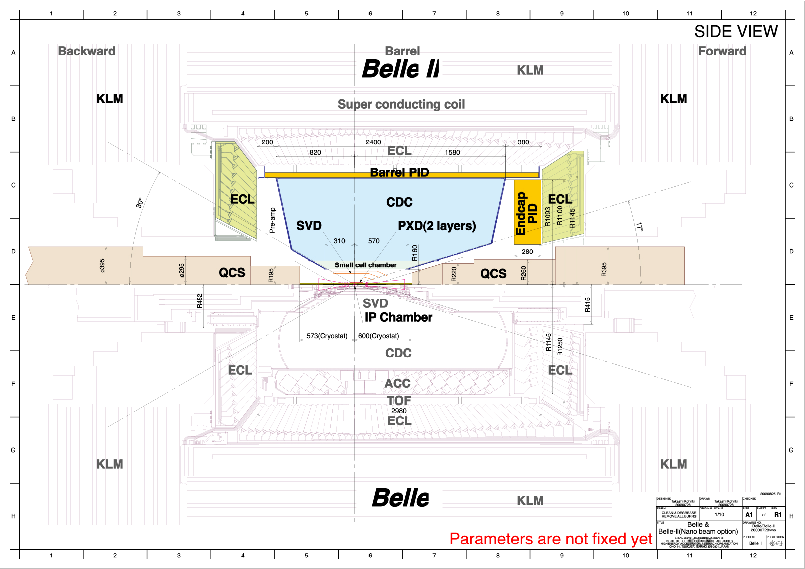
\includegraphics[width=0.5\textwidth]{figures/belle2detector.pdf}
  \caption[Belle II detector to be shown in List of Figure.]{Belle II detector configuration. Get from TDR~\cite{Abe:2010sj}.}
  \label{fig:belledetector}
\end{center}
\end{figure}

If you want to use captions for subfigure in one figure environment, you can use subfigure package as in Fig.~\ref{fig:NTUlogo}.

\begin{figure}[ht]
\centering
    \begin{subfigure}[b]{0.3\textwidth}
        
\includegraphics[width=\textwidth]{figures/NTU_logo_color.pdf}
        \caption{Colored logo.}
    \end{subfigure}
    \hspace{0.2\textwidth}
    \begin{subfigure}[b]{0.3\textwidth}
        
\includegraphics[width=\textwidth]{figures/NTU_logo_gray.pdf}
        \caption{Gray logo.}
    \end{subfigure}
\caption{NTU logo.}
\label{fig:NTUlogo}
\end{figure}

If you are creating figures from {\tt ROOT}, your are advised to use the Belle2 style files from my \href{http://hep5.phys.ntu.edu.tw/indico/event/1174/contribution/8/material/slides/0.pdf}{plotting style workshop}.

\clearpage

\section{Tables}
\label{sec:tab}

A table can be constructed by {\tt tabularx} environment. There are three newly defined column type in this template:\\
{\tt C}: equally share the column width and automatically change line in the text, with center text alignment.\\
{\tt L}: equally share the column width and automatically change line in the text, with left text alignment.\\
{\tt R}: equally share the column width and automatically change line in the text, with right text alignment.

\begin{table}[ht]
\begin{center}
\begin{tabularx}{\textwidth}{c|L|CR}
\hline \hline
This column not sharing width & This column sharing width and automatically change line & This column sharing width and automatically change line &  This column sharing width and automatically change line  \\
\hline 
some table content & \multirow{2}{*}{multirow} & \multicolumn{2}{c}{$M_{bc}=5.29~\text{GeV}/c^2$}    \\
\cline{3-4}
other table content &  & content with \newline line change\gape{\footnotemark} & $-\pi\textnormal{--}-\frac{\pi}{2}$ \\
\hline \hline
\end{tabularx} 
\caption{A simple table contains different contents.}
\label{tab:tab}
\end{center}
\end{table}

\footnotetext{Set footnote like this if you want to add it in a table.}

\section{Equation}

If you want to write some equations in your thesis, you can use {\tt equation} environment, as shown in Eq.~\ref{eqn:eqn} --~\ref{eqn:eqn2}.

\begin{equation}
f(x)=\left\{
\begin{array}{l}
v_{0} + 2\sum\limits_{n=1}^\infty v_{n}\cos{(nx)}, \\
\sum\limits_{n=0}^\infty a_{n}(x)^n + a_{4} \cos{(2x)}, \\
\sum\limits_{n=0}^\infty a_{n}(x)^n.
\end{array} \right.
\label{eqn:eqn}
\end{equation}

\begin{equation}
\begin{aligned}
\int L \text{d}t = &  300~\rm fb^{-1}, \\
% column1 & column2 \\
\int L \text{d}t = &  8\times10^{35}~\text{cm}^{-2} \text{s}^{-1}. 
\end{aligned}
\label{eqn:eqn2}
\end{equation}

Remember that an equation is also included in your paragraph, so don't do extra line break when input an {\tt equation}. For example, this is an equation to be described within a sentence, written as
\begin{equation}
f(\xi)=\xi(\Vec{a}\times\Vec{b})\cdot\Vec{c},
\label{eqn:eqn3}
\end{equation}
and the sentence behind it is not indented. There is a comma behind the equation to claim that there are still some words. For very short equation or math notation, you can directly describe it in line, such as $\Delta E< 0.01~\text{MeV}$ or $p_{\rm T} \ge 0.25~\text{GeV}/c$.
% !TeX root = ../main.tex

\chapter{中文測試}
\label{chp:chinese}

\section{出師表}

臣亮言:先帝創業未半,而中道崩殂。今天下三分,益州疲弊,此誠危急存亡之秋也。然侍衛之臣,不懈於內;忠志之士,忘身於外者,蓋追先帝之殊遇,欲報之於陛下也。誠宜開張聖聽,以光先帝遺德,恢弘志士之氣;不宜妄自菲薄,引喻失義,以塞忠諫之路也。宮中府中,俱為一體,陟罰臧否,不宜異同。若有作姦犯科,及為忠善者,宜付有司,論其刑賞,以昭陛下平明之治,不宜篇私,使內外異法也。\par

侍中、侍郎郭攸之、費褘、董允等,此皆良實,志慮忠純,是以先帝簡拔以遺陛下。愚以為宮中之事,事無大小,悉以咨之,然後施行,必能裨補闕漏,有所廣益。將軍向寵,性行淑均,曉暢軍事,試用於昔日,先帝稱之曰「能」,是以眾議舉寵為督。愚以為營中之事,悉以咨之,必能使行陣和睦,優劣得所。親賢臣,遠小人,此先漢所以興隆也;親小人,遠賢臣,此後漢所以傾頹也。先帝在時,每與臣論此事,未嘗不歎息痛恨於桓、靈也。侍中、尚書、長史;參軍,此悉貞良死節之臣也,願陛下親之信之,則漢室之隆,可計日而待也。

臣本布衣,躬耕於南陽,苟全性命於亂世,不求聞達於諸侯。先帝不以臣卑鄙,猥自枉屈,三顧臣於草廬之中,諮臣以當世之事,由是感激,遂許先帝以驅馳。後值傾覆,受任於敗軍之際,奉命於危難之間,爾來二十有一年矣!先帝知臣謹慎,故臨崩寄臣以大事也。受命以來,夙夜憂勤,恐託付不效,以傷先帝之明。故五月渡瀘,深入不毛。今南方已定,兵甲已足,當獎率三軍,北定中原,庶竭駑鈍,攘除奸凶,興復漢室,還於舊都;此臣所以報先帝而忠陛下之職分也。至於斟酌損益,進盡忠言,則攸之、褘、允之任也。

願陛下託臣以討賊興復之效;不效,則治臣之罪,以告先帝之靈。若無興德之言,則戮允等,以彰其慢。陛下亦宜自課,以諮諏善道,察納雅言,深追先帝遺詔,臣不勝受恩感激。

今當遠離,臨表涕泣,不知所云。

\section{短歌行}

對酒當歌,人生幾何!譬如朝露,去日苦多。
慨當以慷,憂思難忘。何以解憂?唯有杜康。
青青子衿,悠悠我心。但為君故,沉吟至今。
呦呦鹿鳴,食野之苹。我有嘉賓,鼓瑟吹笙。
明明如月,何時可掇?憂從中來,不可斷絕。
越陌度阡,枉用相存。契闊談宴,心念舊恩。
月明星稀,烏鵲南飛。繞樹三匝,何枝可依?
山不厭高,海不厭深。周公吐哺,天下歸心。

\subsection{短歌行}

對酒當歌,人生幾何!譬如朝露,去日苦多。
慨當以慷,憂思難忘。何以解憂?唯有杜康。
青青子衿,悠悠我心。但為君故,沉吟至今。
呦呦鹿鳴,食野之苹。我有嘉賓,鼓瑟吹笙。
明明如月,何時可掇?憂從中來,不可斷絕。
越陌度阡,枉用相存。契闊談宴,心念舊恩。
月明星稀,烏鵲南飛。繞樹三匝,何枝可依?
山不厭高,海不厭深。周公吐哺,天下歸心。
% !TeX root = ../main.tex

\chapter{Other Chapter}

\section{Some section}

\lipsum

\section{Another section}

\lipsum

\subsection{Another subsection}

\lipsum

% 附錄
% Appendices
\appendix
% !TeX root = ../main.tex

\chapter{Lipsum in English}
\label{app:LipsumEng}

\section{Lipsum 01}
\lipsum[1-1]

\section{Lipsum 02}
\lipsum[2-2]

% 參考文獻
% References
\refmatter
\bibliographystyle{aip}
\bibliography{back/references}

\end{document}
